% Supplementary material for docs/paper/medsys-paper.tex.
% Tables and figures are generated by research/supplement_stats.py; compile with
% tectonic -X compile medsys-supplement.tex (or pdflatex twice).
\documentclass[conference]{IEEEtran}

\usepackage{amsmath,amssymb}
\usepackage{graphicx}
\usepackage{booktabs}
\usepackage{array}
\usepackage{xcolor}
\usepackage{url}
\usepackage{xspace}
\usepackage{iftex}
\ifXeTeX
  \usepackage{fontspec}
  \setmainfont{texgyretermes}[Extension=.otf, UprightFont=*-regular, BoldFont=*-bold,
    ItalicFont=*-italic, BoldItalicFont=*-bolditalic]
\fi

\graphicspath{{figures/}}
\newcommand{\lvl}[1]{\texttt{#1}}
\newcommand{\mm}{\,mm\xspace}
\renewcommand{\thetable}{S\arabic{table}}
\renewcommand{\thefigure}{S\arabic{figure}}
\renewcommand{\thesection}{S\arabic{section}}

\begin{document}

\title{Supplementary Material: Stage-Wise Attribution of Geometric Error in Automatic Anatomical Surface Reconstruction From Computed Tomography}

\author{\IEEEauthorblockN{Sameer Morya}
\IEEEauthorblockA{K J Somaiya School of Engineering, Mumbai, India\\ sameer.morya@somaiya.edu}
\and
\IEEEauthorblockN{Sarthak Wage}
\IEEEauthorblockA{K J Somaiya School of Engineering, Mumbai, India\\ sarthak.wage@somaiya.edu}}

\maketitle

\begin{abstract}
This supplement holds the analyses behind the revised paper that do not fit its six pages. Sections S1--S12 each answer one point of the review of the first version and name it; S13 and S14 report two checks made since, on the engine's repeatability and on the accuracy estimate the application derives from these results. Every table and figure is generated from the per-mesh results by \texttt{research/supplement\_stats.py}; the paper's own tables come from \texttt{research/paper\_stats.py}. Organ: spleen (MSD Task09, 41 scans) or the held-out pancreas (MSD Task07, 41 scans drawn at random); TS: TotalSegmentator in fast (3\mm) or full (1.5\mm) mode; canonical: no blur, smoothing or decimation; production: the application's settings.
\end{abstract}

\section{Design and counts}
\emph{Review: clarify design and counts.} Table~\ref{s:counts} counts the units, configurations, engine calls and meshes of every run. Configurations per mask are the 48-point grid (blur $\{0,0.5,1\}$\mm $\times$ Taubin $\{0,10,30,60\}$ $\times$ decimation $\{0,0.25,0.5,0.75\}$), production, and production with blur held at 0.5\mm (production-mm). Engine calls count one segmentation per scan and resolution level a level actually resampled; levels that leave a scan unchanged reuse its native mask. The meshes count every scored mesh; level effects use only the scans a level resampled (spleen: 41 at \lvl{iso1.5} and \lvl{iso3}, 14 at \lvl{slice5}; pancreas: 41, 41 and 35).

\emph{Which comparisons use which settings.} Level effects, Table~II of the paper and the held-out tests H1, H4 and H5 use the canonical configuration. Variance shares (Table~III, H2, H3) use the 48 grid configurations. The grid comparison (H6) pairs native and \lvl{iso3} meshes at identical physical settings across all 48 grid configurations. Closure in Table~II and the deployed-settings results use production; S7 compares production with production-mm.

\begin{table*}[!t]
\caption{Design and counts of every run.}
\label{s:counts}
\centering\footnotesize
\begin{tabular}{lllllrrrr}
\toprule
Tier & Data & Units & Reference & Segmentation & Levels & Configs & Engine calls & Meshes \\
\midrule
Tier 1 & phantoms & 4 shapes $\times$ 5 placements & exact surface & -- & 4 & 97 & -- & 7,760 \\
Tier 2 & Spleen & 41 scans & expert mask & Expert mask, TS fast, TS full & 4 & 50 & 137, 137 & 24,600 \\
 & Pancreas & 41 scans & expert mask & Expert mask, TS fast, TS full & 4 & 50 & 158, 158 & 24,600 \\
Sensitivity & Spleen & 41 scans & expert mask & Expert mask, TS fast & 4 & 3 & 110 & 984 \\
\bottomrule
\end{tabular}

\end{table*}

\section{Tier 1 floor and smoothing by organ}
\emph{Review: phantom interactions may not generalise.} Table~\ref{s:floor} is the canonical error floor on exact surfaces (Table~II of the first version). Table~\ref{s:smooth} tests the interaction the phantoms showed, smoothing that helps compact shapes and harms the thin capsule, on both organs. On anatomy smoothing moves the native expert mesh away from its unsmoothed reference, as it must; on the 3\mm grid light smoothing slightly helps the pancreas expert mask (0.456 to 0.430\mm at 10 iterations) but not the spleen's, heavy smoothing harms both, and engine meshes change by at most 0.19\mm. On the phantoms the reversal between shapes holds without blur or decimation (0.271 to 0.160\mm for the sphere, 0.331 to 0.629\mm for the capsule at 2\mm). The interaction is therefore shape-specific: no organ showed the capsule's doubling of error, although the pancreas is the more sensitive of the two.

\begin{table}[!t]
\caption{Tier~1 error floor: ASSD (HD95) in mm of the canonical reconstruction against the exact surface, mean of five placements.}
\label{s:floor}
\centering\scriptsize
\setlength{\tabcolsep}{2.5pt}
\begin{tabular}{lcccc}
\toprule
Phantom & 0.5\,mm & 1\,mm & 2\,mm & $0.8\times0.8\times5$\,mm \\
\midrule
Sphere & 0.070 (0.17) & 0.147 (0.34) & 0.271 (0.75) & 0.495 (1.62) \\
Capsule & 0.069 (0.17) & 0.144 (0.35) & 0.331 (0.77) & 0.634 (1.95) \\
Torus & 0.068 (0.16) & 0.138 (0.33) & 0.278 (0.66) & 0.499 (1.61) \\
Rounded box & 0.072 (0.17) & 0.145 (0.33) & 0.297 (0.68) & 0.525 (1.72) \\
\bottomrule
\end{tabular}

\end{table}

\begin{table}[!t]
\caption{Mean ASSD (mm) by Taubin iterations without blur or decimation (Lewiner marching cubes for the phantoms).}
\label{s:smooth}
\centering\scriptsize
\setlength{\tabcolsep}{2.5pt}
\begin{tabular}{llrrrr}
\toprule
Surface & Grid & 0 it. & 10 it. & 30 it. & 60 it. \\
\midrule
Phantom: sphere & 1\,mm (exact) & 0.147 & 0.126 & 0.068 & 0.064 \\
 & 2\,mm (exact) & 0.271 & 0.223 & 0.160 & 0.174 \\
Phantom: capsule & 1\,mm (exact) & 0.144 & 0.127 & 0.107 & 0.141 \\
 & 2\,mm (exact) & 0.331 & 0.322 & 0.629 & 1.599 \\
Phantom: torus & 1\,mm (exact) & 0.138 & 0.116 & 0.063 & 0.055 \\
 & 2\,mm (exact) & 0.278 & 0.239 & 0.155 & 0.164 \\
Phantom: rounded box & 1\,mm (exact) & 0.145 & 0.125 & 0.068 & 0.086 \\
 & 2\,mm (exact) & 0.297 & 0.260 & 0.206 & 0.320 \\
\midrule
Spleen: Expert mask & \texttt{native} & 0.000 & 0.046 & 0.215 & 0.306 \\
 & \texttt{iso3} & 0.418 & 0.422 & 0.475 & 0.537 \\
Spleen: TS fast & \texttt{native} & 0.901 & 0.911 & 0.961 & 0.978 \\
 & \texttt{iso3} & 0.907 & 0.920 & 0.929 & 0.919 \\
Spleen: TS full & \texttt{native} & 0.790 & 0.813 & 0.869 & 0.890 \\
 & \texttt{iso3} & 1.210 & 1.226 & 1.215 & 1.193 \\
Pancreas: Expert mask & \texttt{native} & 0.000 & 0.041 & 0.172 & 0.229 \\
 & \texttt{iso3} & 0.456 & 0.430 & 0.437 & 0.553 \\
Pancreas: TS fast & \texttt{native} & 2.722 & 2.752 & 2.827 & 2.873 \\
 & \texttt{iso3} & 2.842 & 2.865 & 2.914 & 2.961 \\
Pancreas: TS full & \texttt{native} & 3.021 & 3.057 & 3.142 & 3.174 \\
 & \texttt{iso3} & 3.507 & 3.550 & 3.628 & 3.693 \\
\bottomrule
\end{tabular}

\end{table}

\section{Per-scan distributions and failure cases}
\emph{Review: report per-scan distributions and failure cases, not only means.} Fig.~\ref{s:perscan} shows every scan's canonical ASSD across levels and Table~\ref{s:perscantab} its median, interquartile range and worst case. Table~\ref{s:fail} lists the three worst scans per engine at native resolution, with the largest connected region the engine missed or added, as a share of the expert organ. The spleen failures are single missed regions (18--20\% of the organ in scan 44); the pancreas failures are missed tumour: scan 415 holds 732\,cm$^3$ of tumour around 135\,cm$^3$ of pancreas, the engine segments the pancreas alone (Dice 0.16), and the merged reference therefore counts the tumour as missed organ. One spleen scan (26) is cut by the field of view; no pancreas scan is. Fig.~\ref{s:maps} shows where the fast engine's error lies on a median spleen scan and on the worst.

\begin{figure*}[!t]
\centering
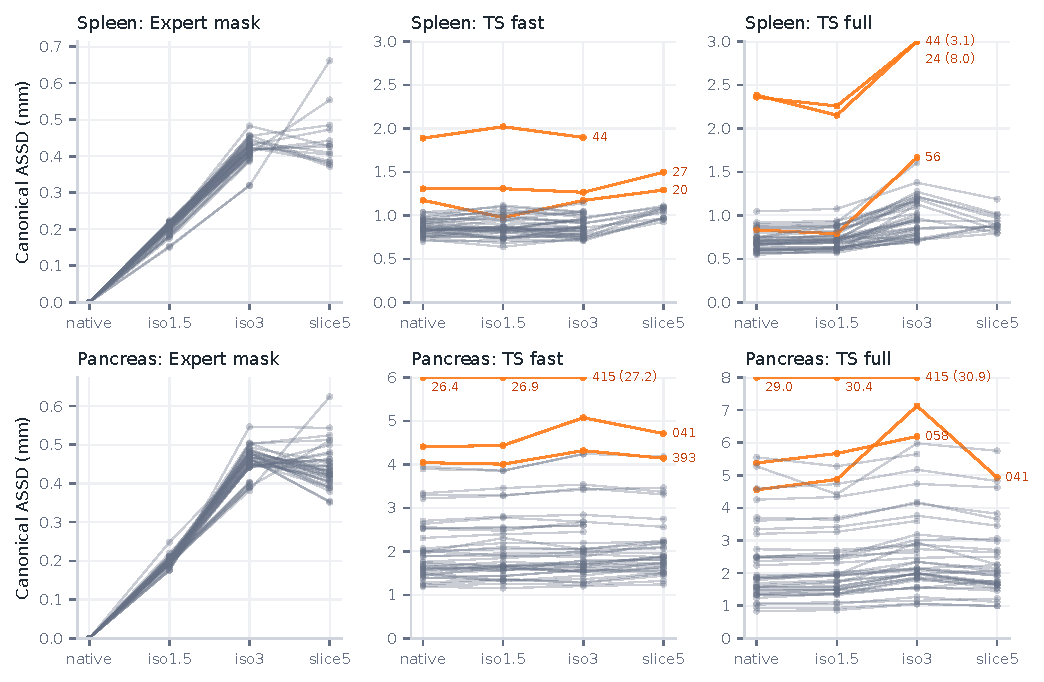
\includegraphics[width=\textwidth]{per_scan.pdf}
\caption{Canonical ASSD of every scan across resolution levels, by organ and mask source. Orange: the three scans with the largest error; numbers in brackets are values above the axis.}
\label{s:perscan}
\end{figure*}

\begin{table}[!t]
\caption{Canonical ASSD across scans: median [IQR] and worst scan (mm).}
\label{s:perscantab}
\centering\scriptsize
\setlength{\tabcolsep}{2.5pt}
\begin{tabular}{lllrrr}
\toprule
Organ & Source & Level & $n$ & Median [IQR] (mm) & Worst (scan) \\
\midrule
Spleen & Expert mask & \texttt{iso1.5} & 41 & 0.207 [0.199, 0.216] & 0.224 (63) \\
 &  & \texttt{iso3} & 41 & 0.418 [0.406, 0.432] & 0.483 (13) \\
 &  & \texttt{slice5} & 14 & 0.427 [0.392, 0.466] & 0.661 (53) \\
 & TS fast & \texttt{native} & 41 & 0.854 [0.810, 0.939] & 1.888 (44) \\
 &  & \texttt{iso1.5} & 41 & 0.848 [0.808, 0.976] & 2.019 (44) \\
 &  & \texttt{iso3} & 41 & 0.858 [0.781, 0.962] & 1.896 (44) \\
 &  & \texttt{slice5} & 14 & 1.061 [0.968, 1.096] & 1.495 (27) \\
 & TS full & \texttt{native} & 41 & 0.699 [0.627, 0.797] & 2.382 (24) \\
 &  & \texttt{iso1.5} & 41 & 0.720 [0.634, 0.819] & 2.257 (44) \\
 &  & \texttt{iso3} & 41 & 0.950 [0.790, 1.173] & 7.966 (24) \\
 &  & \texttt{slice5} & 14 & 0.886 [0.850, 0.961] & 1.186 (20) \\
\midrule
Pancreas & Expert mask & \texttt{iso1.5} & 41 & 0.199 [0.194, 0.204] & 0.248 (075) \\
 &  & \texttt{iso3} & 41 & 0.461 [0.442, 0.478] & 0.546 (339) \\
 &  & \texttt{slice5} & 35 & 0.433 [0.410, 0.462] & 0.624 (120) \\
 & TS fast & \texttt{native} & 41 & 1.881 [1.532, 2.549] & 26.418 (415) \\
 &  & \texttt{iso1.5} & 41 & 1.890 [1.574, 2.554] & 26.919 (415) \\
 &  & \texttt{iso3} & 41 & 1.934 [1.572, 2.679] & 27.187 (415) \\
 &  & \texttt{slice5} & 35 & 1.864 [1.643, 2.234] & 4.709 (041) \\
 & TS full & \texttt{native} & 41 & 1.870 [1.476, 3.203] & 28.976 (415) \\
 &  & \texttt{iso1.5} & 41 & 1.953 [1.492, 3.264] & 30.383 (415) \\
 &  & \texttt{iso3} & 41 & 2.345 [1.869, 3.599] & 30.904 (415) \\
 &  & \texttt{slice5} & 35 & 1.997 [1.643, 2.840] & 5.749 (393) \\
\bottomrule
\end{tabular}

\end{table}

\begin{table*}[!t]
\caption{The three worst scans per engine at native resolution (canonical mesh). Missed and extra: largest connected region the engine missed or added, as \% of the expert organ volume.}
\label{s:fail}
\centering\footnotesize
\begin{tabular}{lllrrrrrrr}
\toprule
Organ & Engine & Scan & Slice (mm) & Dice & ASSD (mm) & HD95 (mm) & Missed (\%) & Extra (\%) & Volume (\%) \\
\midrule
Spleen & TS fast & 44 & 5 & 0.851 & 1.89 & 8.6 & 18.2 & 4.8 & -9.7 \\
 &  & 27 & 4 & 0.923 & 1.30 & 10.6 & 1.5 & 4.3 & +1.0 \\
 &  & 20 & 1.5 & 0.933 & 1.17 & 3.1 & 4.9 & 5.9 & -0.0 \\
\midrule
Spleen & TS full & 24 & 5 & 0.892 & 2.38 & 5.5 & 7.4 & 1.5 & -9.1 \\
 &  & 44 & 5 & 0.852 & 2.36 & 18.9 & 19.5 & 3.6 & -13.7 \\
 &  & 20 & 1.5 & 0.944 & 1.05 & 2.8 & 4.2 & 2.7 & -1.1 \\
\midrule
Pancreas & TS fast & 415 & 5 & 0.163 & 26.42 & 109.1 & 90.2 & 0.6 & -89.7 \\
 &  & 041 & 1.5 & 0.575 & 4.40 & 17.1 & 58.7 & 2.1 & -56.5 \\
 &  & 393 & 2.5 & 0.534 & 4.04 & 17.7 & 50.0 & 0.5 & -61.7 \\
\midrule
Pancreas & TS full & 415 & 5 & 0.137 & 28.98 & 116.7 & 91.7 & 0.5 & -91.7 \\
 &  & 365 & 5 & 0.647 & 5.55 & 41.8 & 35.0 & 0.9 & -46.8 \\
 &  & 058 & 5 & 0.546 & 5.38 & 33.2 & 60.7 & 2.0 & -59.6 \\
\bottomrule
\end{tabular}

\end{table*}

\begin{figure}[!t]
\centering
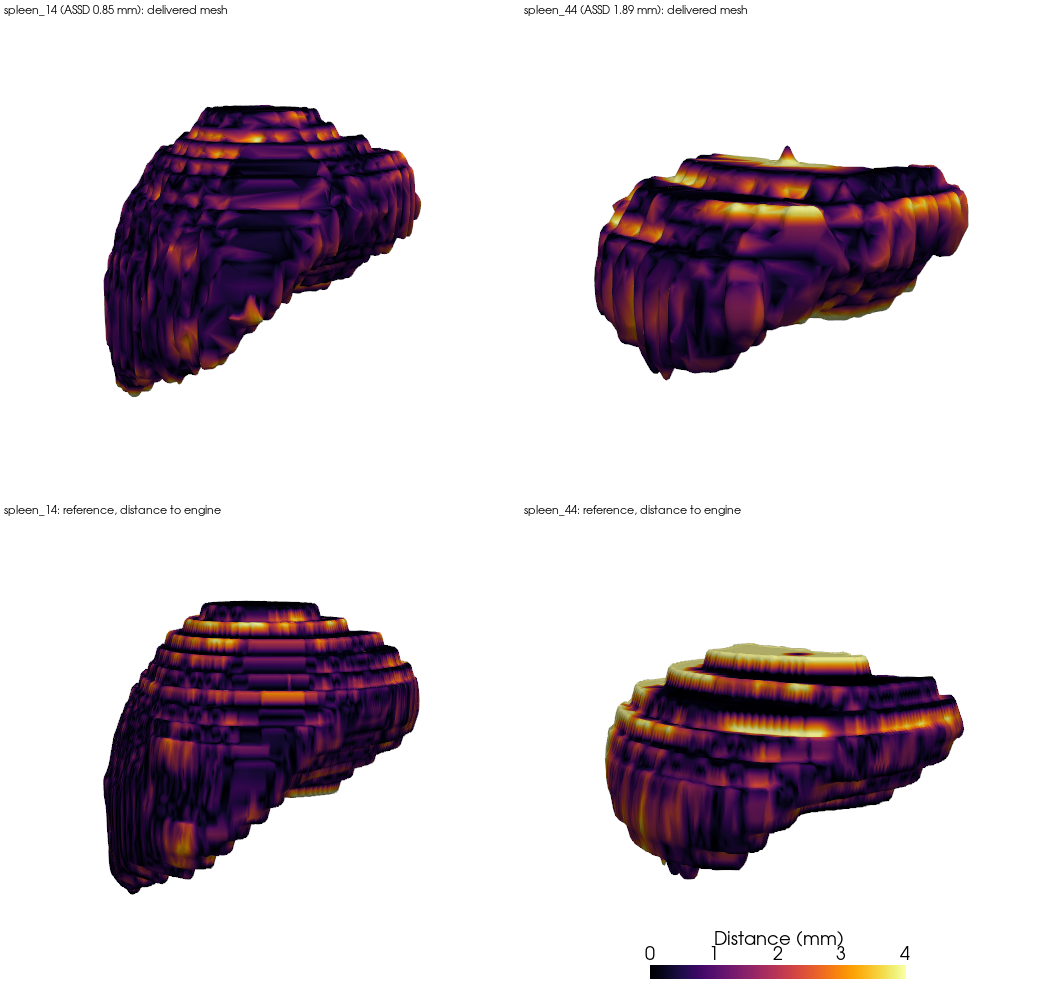
\includegraphics[width=\columnwidth]{error_maps.png}
\caption{Local error of TS fast on a median spleen scan (14) and the worst (44), coronal view. Top: the delivered production mesh coloured by its distance to the reference (added or displaced surface). Bottom: the reference coloured by its distance to the engine's mesh (missed anatomy); the bright block in scan 44 is the missed 18\% of the organ.}
\label{s:maps}
\end{figure}

\section{Sampling models and prediction intervals}
\emph{Review: refine the empirical model; validate slice-only coarsening; report prediction intervals.} Table~\ref{s:models} compares the paper's model M0 with three refinements on the spleen's 96 resampled expert masks, by leave-one-scan-out error, a 95\% prediction interval (the 95th percentile of the absolute leave-one-scan-out residuals), the error when \lvl{slice5} is held out of the fit, and transfer to the held-out pancreas and to the box slice profile. A free intercept (M1) fits slightly better but cannot be trusted outside the fitted range: holding out \lvl{iso1.5} it misses by 0.28\mm. Linear axis terms (M2) fit worse, and quadrature axis weights (M3) converge to equal values (0.031 and 0.032), so the pooled $\Delta$ is the right form. M0's prediction interval of $\pm0.111$\mm covers 98\% of pancreas points, and its slope is 0.177 [0.171, 0.184] on the spleen, 0.180 [0.176, 0.184] on the pancreas and 0.174 [0.167, 0.181] with the box profile. Slice-only coarsening remains the weakest prediction (0.109\mm when \lvl{slice5} is held out), because the spleen has 14 such scans and they span 1.5--4\mm native slices.

\begin{table*}[!t]
\caption{Sampling models for the canonical ASSD (mm) of the resampled expert mask. Coefficients in mm per mm ($c$ in mm$^0$); PI: 95\% prediction interval; PI cov.: share of pancreas points inside the spleen PI.}
\label{s:models}
\centering\footnotesize
\begin{tabular}{lrrrrrrr}
\toprule
Model & Coefficients & $R^2$ & LOSO MAE & 95\% PI & slice5 held out & Pancreas MAE (PI cov.) & Box profile MAE \\
\midrule
M0: $b\Delta$ & 0.177 & 0.76 & 0.037 & $\pm$0.111 & 0.109 & 0.030 (98\%) & 0.045 \\
M1: $a+b\Delta$ & 0.066, 0.145 & 0.80 & 0.030 & $\pm$0.093 & 0.099 & 0.030 (96\%) & 0.041 \\
M2: $b_1\Delta_{\mathrm{in}}+b_2\Delta_{\mathrm{sl}}$ & 0.165, 0.159 & 0.54 & 0.056 & $\pm$0.205 & 0.414 & 0.051 (98\%) & 0.067 \\
M3: $\sqrt{c_1\Delta_{\mathrm{in}}^2+c_2\Delta_{\mathrm{sl}}^2}$ & 0.031, 0.032 & 0.76 & 0.039 & $\pm$0.120 & 0.254 & 0.030 (98\%) & 0.045 \\
\bottomrule
\end{tabular}

\end{table*}

\section{The slice5 subsets}
\emph{Review: the 14-scan subset limits power; report per-scan effects and sensitivity.} Table~\ref{s:slice5} gives each \lvl{slice5} effect with its leave-one-scan-out range, the number of scans whose error rose, and the minimum effect detectable with 80\% power at $\alpha=0.05$ (paired $t$ approximation). Every spleen scan rose for every source, no single scan moves an effect by more than 0.02\mm, and the observed effects are about three times the detectable minimum. The pancreas, with 35 resampled scans, replicates the effect.

\begin{table*}[!t]
\caption{Paired change in canonical ASSD from native to \lvl{slice5} (mm). MDE: minimum detectable effect, 80\% power.}
\label{s:slice5}
\centering\footnotesize
\begin{tabular}{llrrrrrr}
\toprule
Organ & Source & $n$ & Change [95\% CI] (mm) & Leave-one-out range & Scans up & SD & MDE$_{80\%}$ \\
\midrule
Spleen & Expert mask & 14 & +0.445 [+0.410, +0.489] & +0.429 to +0.451 & 14/14 & 0.079 & 0.064 \\
 & TS fast & 14 & +0.188 [+0.152, +0.228] & +0.175 to +0.195 & 14/14 & 0.078 & 0.063 \\
 & TS full & 14 & +0.212 [+0.173, +0.251] & +0.201 to +0.219 & 14/14 & 0.078 & 0.063 \\
\midrule
Pancreas & Expert mask & 35 & +0.442 [+0.425, +0.461] & +0.437 to +0.445 & 35/35 & 0.055 & 0.027 \\
 & TS fast & 35 & +0.143 [+0.116, +0.170] & +0.138 to +0.149 & 34/35 & 0.083 & 0.040 \\
 & TS full & 35 & +0.232 [+0.178, +0.285] & +0.221 to +0.240 & 32/35 & 0.162 & 0.079 \\
\bottomrule
\end{tabular}

\end{table*}

\section{Topology without the field-of-view-cut scan}
\emph{Review: one cut scan caps the topology curves.} Table~\ref{s:topo} repeats the closure rates with spleen scan 26 removed. Without decimation every mesh is then closed; the effect of decimation on closure is unchanged.

\begin{table*}[!t]
\caption{Share of closed meshes (\%) over the grid by decimation: all scans / without the field-of-view-cut scan.}
\label{s:topo}
\centering\footnotesize
\begin{tabular}{lllrrrr}
\toprule
& & & \multicolumn{4}{c}{Closed (\%), all scans / without FOV-cut scans, by decimation} \\
\cmidrule(lr){4-7}
Organ & Source & Level & 0 & 0.25 & 0.5 & 0.75 \\
\midrule
Spleen & Expert mask & \texttt{native} & 98 / 100 & 96 / 99 & 90 / 92 & 68 / 70 \\
 &  & \texttt{iso1.5} & 98 / 100 & 95 / 97 & 92 / 94 & 75 / 77 \\
 &  & \texttt{iso3} & 98 / 100 & 97 / 99 & 93 / 96 & 79 / 81 \\
 &  & \texttt{slice5} & 100 / 100 & 100 / 100 & 93 / 93 & 71 / 71 \\
\midrule
Spleen & TS fast & \texttt{native} & 98 / 100 & 97 / 100 & 93 / 95 & 57 / 59 \\
 &  & \texttt{iso1.5} & 98 / 100 & 98 / 100 & 93 / 95 & 63 / 65 \\
 &  & \texttt{iso3} & 98 / 100 & 95 / 97 & 94 / 96 & 83 / 85 \\
 &  & \texttt{slice5} & 100 / 100 & 99 / 99 & 95 / 95 & 58 / 58 \\
\midrule
Spleen & TS full & \texttt{native} & 98 / 100 & 96 / 99 & 89 / 91 & 58 / 59 \\
 &  & \texttt{iso1.5} & 98 / 100 & 93 / 96 & 89 / 91 & 67 / 69 \\
 &  & \texttt{iso3} & 98 / 100 & 94 / 96 & 92 / 94 & 82 / 84 \\
 &  & \texttt{slice5} & 100 / 100 & 100 / 100 & 95 / 95 & 54 / 54 \\
\midrule
Pancreas & Expert mask & \texttt{native} & 100 / 100 & 96 / 96 & 90 / 90 & 58 / 58 \\
 &  & \texttt{iso1.5} & 100 / 100 & 98 / 98 & 93 / 93 & 71 / 71 \\
 &  & \texttt{iso3} & 100 / 100 & 98 / 98 & 95 / 95 & 85 / 85 \\
 &  & \texttt{slice5} & 100 / 100 & 100 / 100 & 94 / 94 & 66 / 66 \\
\midrule
Pancreas & TS fast & \texttt{native} & 100 / 100 & 98 / 98 & 86 / 86 & 38 / 38 \\
 &  & \texttt{iso1.5} & 99 / 99 & 95 / 95 & 86 / 86 & 51 / 51 \\
 &  & \texttt{iso3} & 100 / 100 & 96 / 96 & 89 / 89 & 63 / 63 \\
 &  & \texttt{slice5} & 100 / 100 & 94 / 94 & 88 / 88 & 49 / 49 \\
\midrule
Pancreas & TS full & \texttt{native} & 100 / 100 & 94 / 94 & 75 / 75 & 38 / 38 \\
 &  & \texttt{iso1.5} & 100 / 100 & 94 / 94 & 83 / 83 & 54 / 54 \\
 &  & \texttt{iso3} & 100 / 100 & 96 / 96 & 90 / 90 & 64 / 64 \\
 &  & \texttt{slice5} & 100 / 100 & 97 / 97 & 84 / 84 & 41 / 41 \\
\bottomrule
\end{tabular}

\end{table*}

\section{Blur in voxels and in millimetres}
\emph{Review: production blur is in voxels, research blur in millimetres.} Table~\ref{s:blur} compares production (0.6 voxels) with production-mm (0.5\mm, same smoothing and decimation) at every level. The two differ most on coarse grids, where 0.6 voxels becomes 1.8\mm: on the expert masks by at most 0.065\mm, on the engines by at most 0.14\mm (TS full, pancreas, \lvl{iso3}). The paper's grid comparison (H6) already holds blur in millimetres.

\begin{table*}[!t]
\caption{Production ASSD (mm) with blur in voxels and in millimetres, paired by scan; closed: \% of closed meshes, voxel / mm.}
\label{s:blur}
\centering\footnotesize
\begin{tabular}{lllrrrrr}
\toprule
Organ & Source & Level & $n$ & Voxel blur & mm blur & mm $-$ voxel [95\% CI] & Closed (\%) \\
\midrule
Spleen & Expert mask & \texttt{native} & 41 & 0.234 & 0.226 & -0.008 [-0.010, -0.006] & 98 / 95 \\
 &  & \texttt{iso1.5} & 41 & 0.374 & 0.358 & -0.016 [-0.019, -0.013] & 95 / 98 \\
 &  & \texttt{iso3} & 41 & 0.517 & 0.486 & -0.031 [-0.035, -0.028] & 98 / 95 \\
 &  & \texttt{slice5} & 14 & 0.425 & 0.417 & -0.008 [-0.012, -0.004] & 93 / 100 \\
\midrule
Spleen & TS fast & \texttt{native} & 41 & 0.948 & 0.956 & +0.008 [+0.004, +0.011] & 66 / 51 \\
 &  & \texttt{iso1.5} & 41 & 0.958 & 0.973 & +0.016 [+0.011, +0.020] & 90 / 90 \\
 &  & \texttt{iso3} & 41 & 0.914 & 0.933 & +0.018 [+0.011, +0.025] & 95 / 98 \\
 &  & \texttt{slice5} & 14 & 1.048 & 1.058 & +0.009 [+0.004, +0.014] & 50 / 64 \\
\midrule
Spleen & TS full & \texttt{native} & 41 & 0.855 & 0.866 & +0.010 [+0.004, +0.020] & 98 / 93 \\
 &  & \texttt{iso1.5} & 41 & 0.860 & 0.878 & +0.017 [+0.007, +0.034] & 93 / 88 \\
 &  & \texttt{iso3} & 41 & 1.205 & 1.229 & +0.024 [-0.026, +0.113] & 95 / 85 \\
 &  & \texttt{slice5} & 14 & 0.899 & 0.907 & +0.008 [+0.004, +0.013] & 86 / 86 \\
\midrule
Pancreas & Expert mask & \texttt{native} & 41 & 0.189 & 0.182 & -0.007 [-0.009, -0.006] & 98 / 95 \\
 &  & \texttt{iso1.5} & 41 & 0.293 & 0.277 & -0.016 [-0.019, -0.013] & 95 / 93 \\
 &  & \texttt{iso3} & 41 & 0.535 & 0.470 & -0.065 [-0.074, -0.056] & 100 / 95 \\
 &  & \texttt{slice5} & 35 & 0.423 & 0.399 & -0.024 [-0.027, -0.021] & 94 / 94 \\
\midrule
Pancreas & TS fast & \texttt{native} & 41 & 2.836 & 2.837 & +0.001 [-0.008, +0.011] & 37 / 66 \\
 &  & \texttt{iso1.5} & 41 & 2.911 & 2.887 & -0.024 [-0.039, -0.010] & 85 / 78 \\
 &  & \texttt{iso3} & 41 & 2.977 & 2.931 & -0.046 [-0.069, -0.022] & 93 / 90 \\
 &  & \texttt{slice5} & 35 & 2.268 & 2.257 & -0.011 [-0.023, +0.002] & 54 / 57 \\
\midrule
Pancreas & TS full & \texttt{native} & 41 & 3.163 & 3.147 & -0.016 [-0.033, +0.002] & 76 / 71 \\
 &  & \texttt{iso1.5} & 41 & 3.222 & 3.196 & -0.026 [-0.039, -0.015] & 93 / 80 \\
 &  & \texttt{iso3} & 41 & 3.796 & 3.659 & -0.137 [-0.194, -0.090] & 90 / 80 \\
 &  & \texttt{slice5} & 35 & 2.529 & 2.490 & -0.039 [-0.065, -0.018] & 77 / 74 \\
\bottomrule
\end{tabular}

\end{table*}

\section{Local and task-specific metrics}
\emph{Review: global metrics hide local defects; add tolerances.} Table~\ref{s:local} adds NSD at 0.5, 1 and 2\mm, the larger directed 99th percentile (P99), the share of the delivered surface in local defects (faces more than 2\mm from the reference) with the largest connected patch (mm$^2$), the mean absolute volume error, and the share of meshes meeting two illustrative tolerances, HD95 $\leq2$\mm and $|$volume error$|\leq5\%$. Resampled expert masks have defects only at \lvl{slice5}, on 0.2--0.7\% of their surface; the engines have defects on 5--9\% of the spleen surface and 27--29\% of the pancreas surface, and on the pancreas fewer than 10\% of engine meshes stay within 5\% of the reference volume. The tolerances are examples, not validated clinical limits.

\begin{table*}[!t]
\caption{Local and task-specific metrics (means over scans; P99 in mm; HD95 $\leq$ 2 and $|$Vol$|\leq$ 5\%: \% of meshes meeting the tolerance). Cfg: canonical or production.}
\label{s:local}
\centering\scriptsize
\setlength{\tabcolsep}{3pt}
\begin{tabular}{llllrrrrrrrrr}
\toprule
Organ & Source & Level & Cfg & NSD$_{0.5}$ & NSD$_1$ & NSD$_2$ & P99 & Defect (\%) & Max patch & $|$Vol$|$ (\%) & HD95$\leq$2 & $|$Vol$|\leq$5\% \\
\midrule
Spleen & Expert mask & \texttt{native} & prod. & 0.88 & 1.00 & 1.00 & 0.87 & 0.0 & 0 & 0.3 & 100 & 100 \\
 &  & \texttt{iso1.5} & cano. & 0.90 & 1.00 & 1.00 & 0.78 & 0.0 & 0 & 0.1 & 100 & 100 \\
 &  & \texttt{iso1.5} & prod. & 0.73 & 0.94 & 1.00 & 1.38 & 0.0 & 0 & 0.7 & 100 & 100 \\
 &  & \texttt{iso3} & cano. & 0.64 & 0.92 & 1.00 & 1.54 & 0.0 & 0 & 0.6 & 100 & 100 \\
 &  & \texttt{iso3} & prod. & 0.60 & 0.86 & 0.99 & 1.96 & 0.0 & 0 & 2.0 & 93 & 98 \\
 &  & \texttt{slice5} & cano. & 0.70 & 0.85 & 0.99 & 1.90 & 0.7 & 756 & 0.8 & 100 & 100 \\
 &  & \texttt{slice5} & prod. & 0.72 & 0.88 & 0.99 & 1.92 & 0.5 & 452 & 1.0 & 93 & 100 \\
\midrule
Spleen & TS fast & \texttt{native} & cano. & 0.41 & 0.66 & 0.89 & 4.98 & 8.9 & 2188 & 2.9 & 0 & 80 \\
 &  & \texttt{native} & prod. & 0.40 & 0.64 & 0.89 & 4.87 & 5.0 & 1740 & 2.7 & 0 & 85 \\
 &  & \texttt{iso1.5} & cano. & 0.42 & 0.65 & 0.90 & 4.78 & 6.5 & 2119 & 2.7 & 0 & 88 \\
 &  & \texttt{iso1.5} & prod. & 0.38 & 0.64 & 0.90 & 4.76 & 3.3 & 1359 & 2.6 & 2 & 88 \\
 &  & \texttt{iso3} & cano. & 0.41 & 0.65 & 0.90 & 4.79 & 4.3 & 1649 & 2.7 & 2 & 83 \\
 &  & \texttt{iso3} & prod. & 0.38 & 0.66 & 0.91 & 4.54 & 1.8 & 1099 & 2.5 & 15 & 88 \\
 &  & \texttt{slice5} & cano. & 0.31 & 0.58 & 0.88 & 5.32 & 8.8 & 2122 & 2.7 & 0 & 86 \\
 &  & \texttt{slice5} & prod. & 0.32 & 0.59 & 0.88 & 5.15 & 6.2 & 1687 & 2.7 & 0 & 86 \\
\midrule
Spleen & TS full & \texttt{native} & cano. & 0.47 & 0.74 & 0.93 & 6.03 & 5.0 & 1207 & 2.9 & 17 & 83 \\
 &  & \texttt{native} & prod. & 0.45 & 0.70 & 0.92 & 6.05 & 3.1 & 950 & 2.8 & 12 & 83 \\
 &  & \texttt{iso1.5} & cano. & 0.49 & 0.72 & 0.92 & 5.92 & 4.0 & 1056 & 2.9 & 15 & 85 \\
 &  & \texttt{iso1.5} & prod. & 0.43 & 0.70 & 0.92 & 4.76 & 2.1 & 801 & 2.9 & 15 & 80 \\
 &  & \texttt{iso3} & cano. & 0.38 & 0.61 & 0.87 & 8.03 & 5.8 & 2613 & 5.9 & 7 & 59 \\
 &  & \texttt{iso3} & prod. & 0.33 & 0.59 & 0.86 & 6.75 & 3.1 & 1346 & 7.4 & 7 & 39 \\
 &  & \texttt{slice5} & cano. & 0.36 & 0.64 & 0.91 & 3.69 & 5.0 & 804 & 3.9 & 0 & 79 \\
 &  & \texttt{slice5} & prod. & 0.37 & 0.64 & 0.91 & 3.60 & 4.0 & 894 & 3.9 & 0 & 71 \\
\midrule
Pancreas & Expert mask & \texttt{native} & prod. & 0.94 & 1.00 & 1.00 & 0.73 & 0.0 & 0 & 0.7 & 100 & 100 \\
 &  & \texttt{iso1.5} & cano. & 0.92 & 1.00 & 1.00 & 0.73 & 0.0 & 0 & 0.4 & 100 & 100 \\
 &  & \texttt{iso1.5} & prod. & 0.82 & 0.98 & 1.00 & 1.08 & 0.0 & 0 & 1.7 & 100 & 100 \\
 &  & \texttt{iso3} & cano. & 0.61 & 0.92 & 1.00 & 1.43 & 0.0 & 0 & 2.2 & 100 & 98 \\
 &  & \texttt{iso3} & prod. & 0.57 & 0.86 & 0.99 & 2.23 & 0.0 & 0 & 6.2 & 98 & 44 \\
 &  & \texttt{slice5} & cano. & 0.67 & 0.81 & 1.00 & 1.39 & 0.2 & 322 & 0.8 & 97 & 100 \\
 &  & \texttt{slice5} & prod. & 0.72 & 0.86 & 1.00 & 1.61 & 0.2 & 203 & 1.9 & 97 & 97 \\
\midrule
Pancreas & TS fast & \texttt{native} & cano. & 0.23 & 0.41 & 0.64 & 15.64 & 29.2 & 12147 & 25.6 & 0 & 10 \\
 &  & \texttt{native} & prod. & 0.21 & 0.38 & 0.63 & 15.92 & 24.0 & 8605 & 25.8 & 0 & 10 \\
 &  & \texttt{iso1.5} & cano. & 0.23 & 0.39 & 0.63 & 15.60 & 27.0 & 10998 & 26.6 & 0 & 10 \\
 &  & \texttt{iso1.5} & prod. & 0.20 & 0.36 & 0.62 & 16.01 & 21.7 & 8328 & 26.8 & 0 & 10 \\
 &  & \texttt{iso3} & cano. & 0.20 & 0.38 & 0.64 & 15.90 & 22.6 & 9495 & 26.3 & 0 & 7 \\
 &  & \texttt{iso3} & prod. & 0.19 & 0.36 & 0.61 & 16.31 & 18.0 & 8619 & 27.4 & 0 & 2 \\
 &  & \texttt{slice5} & cano. & 0.18 & 0.35 & 0.65 & 12.01 & 26.5 & 9462 & 25.3 & 0 & 9 \\
 &  & \texttt{slice5} & prod. & 0.18 & 0.34 & 0.62 & 12.28 & 24.7 & 8482 & 25.5 & 0 & 9 \\
\midrule
Pancreas & TS full & \texttt{native} & cano. & 0.24 & 0.42 & 0.64 & 18.34 & 26.9 & 12191 & 30.8 & 0 & 7 \\
 &  & \texttt{native} & prod. & 0.22 & 0.39 & 0.62 & 18.74 & 23.5 & 9898 & 31.1 & 0 & 7 \\
 &  & \texttt{iso1.5} & cano. & 0.24 & 0.40 & 0.63 & 18.17 & 25.4 & 10482 & 30.8 & 0 & 7 \\
 &  & \texttt{iso1.5} & prod. & 0.21 & 0.37 & 0.62 & 18.60 & 20.8 & 9111 & 31.5 & 0 & 10 \\
 &  & \texttt{iso3} & cano. & 0.18 & 0.34 & 0.58 & 20.17 & 24.7 & 8152 & 34.4 & 0 & 12 \\
 &  & \texttt{iso3} & prod. & 0.16 & 0.31 & 0.54 & 21.45 & 21.1 & 6704 & 37.2 & 0 & 12 \\
 &  & \texttt{slice5} & cano. & 0.18 & 0.35 & 0.65 & 14.83 & 23.9 & 10864 & 29.7 & 0 & 9 \\
 &  & \texttt{slice5} & prod. & 0.18 & 0.34 & 0.62 & 15.31 & 23.2 & 9235 & 30.2 & 0 & 9 \\
\bottomrule
\end{tabular}

\end{table*}

\section{Coarsening-model sensitivity}
\emph{Review: resampling does not reproduce real acquisitions.} The spleen run was repeated at \lvl{iso3} and \lvl{slice5} with a rectangular slice profile one coarse voxel wide (a slab average, applied to the CT and the expert mask) and, for the engine, with white noise of SD 20\,HU added to the Gaussian-coarsened CT (Table~\ref{s:coarse}). The expert mask's sampling error changed by at most 0.003\mm, and the fast engine's error by at most 0.020\mm, about 2\% of its value, with Dice unchanged. These bracket two simulation choices; they do not replace thin and thick reconstructions of the same acquisition, which this dataset does not contain.

\begin{table*}[!t]
\caption{Canonical and production ASSD (mm) under the Gaussian coarsening of the paper and under each variant, paired by scan; Dice G / V: Gaussian / variant.}
\label{s:coarse}
\centering\footnotesize
\begin{tabular}{llllrrrrr}
\toprule
Source & Level & Variant & Config & $n$ & Gaussian & Variant & Difference [95\% CI] & Dice G / V \\
\midrule
Expert mask & \texttt{iso3} & box & canonical & 41 & 0.418 & 0.417 & -0.001 [-0.002, -0.000] & 0.968 / 0.968 \\
 &  & box & production & 41 & 0.517 & 0.518 & +0.001 [-0.001, +0.003] & 0.968 / 0.968 \\
 & \texttt{slice5} & box & canonical & 14 & 0.445 & 0.446 & +0.001 [-0.001, +0.003] & 0.971 / 0.971 \\
 &  & box & production & 14 & 0.425 & 0.427 & +0.003 [+0.001, +0.005] & 0.971 / 0.971 \\
\midrule
TS fast & \texttt{iso3} & box & canonical & 41 & 0.907 & 0.914 & +0.006 [+0.003, +0.010] & 0.940 / 0.940 \\
 &  & box & production & 41 & 0.914 & 0.919 & +0.005 [+0.000, +0.010] & 0.940 / 0.940 \\
 &  & noise & canonical & 41 & 0.907 & 0.926 & +0.019 [+0.007, +0.031] & 0.940 / 0.939 \\
 &  & noise & production & 41 & 0.914 & 0.934 & +0.019 [+0.008, +0.033] & 0.940 / 0.939 \\
 & \texttt{slice5} & box & canonical & 14 & 1.079 & 1.095 & +0.016 [+0.004, +0.027] & 0.926 / 0.925 \\
 &  & box & production & 14 & 1.048 & 1.069 & +0.020 [+0.006, +0.035] & 0.926 / 0.925 \\
 &  & noise & canonical & 14 & 1.079 & 1.081 & +0.002 [-0.010, +0.014] & 0.926 / 0.926 \\
 &  & noise & production & 14 & 1.048 & 1.048 & -0.000 [-0.015, +0.015] & 0.926 / 0.926 \\
\bottomrule
\end{tabular}

\end{table*}

\section{Engine modes}
\emph{Review: test full-resolution mode; is patient dominance fast-mode-specific?} Table~\ref{s:engines} pairs the two modes scan by scan. On the spleen, full mode is more accurate at native, \lvl{iso1.5} and \lvl{slice5} resolution but much worse on 3\mm input; on the pancreas it is worse at every level. Scans still dominate full mode's variance (spleen 59.3\%, pancreas 99.4\%; random intercept 59.6\% and 99.5\%), but on the spleen interactions between scan and resolution take a third of it, because the 3\mm penalty differs between scans. Resolution insensitivity is thus specific to the fast mode on the spleen, and scan dominance holds for both modes.

\begin{table*}[!t]
\caption{TotalSegmentator full against fast mode, paired by scan (ASSD in mm; full better: scans with lower full-mode ASSD).}
\label{s:engines}
\centering\footnotesize
\begin{tabular}{lllrrrrrr}
\toprule
Organ & Level & Config & $n$ & Dice fast / full & ASSD fast & ASSD full & Full $-$ fast [95\% CI] & Full better \\
\midrule
Spleen & \texttt{native} & canonical & 41 & 0.940 / 0.951 & 0.901 & 0.790 & -0.111 [-0.182, -0.009] & 39/41 \\
 &  & production & 41 & 0.940 / 0.951 & 0.948 & 0.855 & -0.093 [-0.150, -0.017] & 37/41 \\
 & \texttt{iso1.5} & canonical & 41 & 0.940 / 0.951 & 0.905 & 0.805 & -0.101 [-0.164, -0.008] & 37/41 \\
 &  & production & 41 & 0.940 / 0.951 & 0.958 & 0.860 & -0.097 [-0.143, -0.047] & 31/41 \\
 & \texttt{iso3} & canonical & 41 & 0.940 / 0.932 & 0.907 & 1.210 & +0.302 [+0.083, +0.689] & 12/41 \\
 &  & production & 41 & 0.940 / 0.932 & 0.914 & 1.205 & +0.291 [+0.135, +0.545] & 3/41 \\
 & \texttt{slice5} & canonical & 14 & 0.926 / 0.937 & 1.079 & 0.913 & -0.165 [-0.225, -0.121] & 14/14 \\
 &  & production & 14 & 0.926 / 0.937 & 1.048 & 0.899 & -0.150 [-0.207, -0.105] & 14/14 \\
\midrule
Pancreas & \texttt{native} & canonical & 41 & 0.753 / 0.738 & 2.722 & 3.021 & +0.298 [+0.087, +0.539] & 18/41 \\
 &  & production & 41 & 0.753 / 0.738 & 2.836 & 3.163 & +0.327 [+0.118, +0.568] & 17/41 \\
 & \texttt{iso1.5} & canonical & 41 & 0.751 / 0.737 & 2.768 & 3.092 & +0.324 [+0.102, +0.598] & 15/41 \\
 &  & production & 41 & 0.751 / 0.737 & 2.911 & 3.222 & +0.311 [+0.084, +0.580] & 14/41 \\
 & \texttt{iso3} & canonical & 41 & 0.753 / 0.698 & 2.842 & 3.507 & +0.665 [+0.417, +0.943] & 5/41 \\
 &  & production & 41 & 0.753 / 0.698 & 2.977 & 3.796 & +0.819 [+0.549, +1.134] & 5/41 \\
 & \texttt{slice5} & canonical & 35 & 0.747 / 0.731 & 2.181 & 2.396 & +0.215 [+0.051, +0.394] & 13/35 \\
 &  & production & 35 & 0.747 / 0.731 & 2.268 & 2.529 & +0.261 [+0.073, +0.457] & 14/35 \\
\bottomrule
\end{tabular}

\end{table*}

\section{Scan properties behind the case effect}
\emph{Review: case difficulty is inferred, not measured.} Table~\ref{s:cov} correlates each scan's native canonical engine ASSD with measured properties: native spacing, expert organ volume, mean and SD of the organ's HU (eroded by one voxel), organ-to-surround contrast (organ mean HU minus that of a 3\mm soft-tissue shell around it), boundary-to-volume ratio and whether the organ touches the image edge; the last column is the leave-one-scan-out $R^2$ of a linear model on the continuous properties. Low contrast goes with higher error on both organs. On the spleen these properties explain little ($R^2\approx0.15$); on the pancreas, label volume, which here measures tumour burden, explains much more ($R^2$ 0.59 and 0.76). The paper therefore calls the case effect between-scan variation and does not claim to have measured difficulty.

\begin{table*}[!t]
\caption{Spearman correlation of native canonical engine ASSD with scan properties ($^*$: $p<0.05$, uncorrected), and leave-one-scan-out $R^2$ of a linear model.}
\label{s:cov}
\centering\scriptsize
\setlength{\tabcolsep}{3pt}
\begin{tabular}{llrrrrrrrrr}
\toprule
Organ & Engine & Slice spacing & In-plane spacing & Organ volume & Organ HU & Organ HU SD & Organ-to-surround contrast & Boundary-to-volume ratio & Cut by field of view & LOSO $R^2$ \\
\midrule
Spleen & TS fast & +0.16 & -0.02 & -0.03 & +0.21 & -0.05 & -0.59$^*$ & +0.05 & -0.09 & 0.14 \\
 & TS full & +0.20 & -0.06 & -0.14 & -0.03 & -0.13 & -0.59$^*$ & +0.11 & -0.01 & 0.15 \\
Pancreas & TS fast & +0.20 & +0.11 & +0.49$^*$ & -0.36$^*$ & -0.01 & -0.49$^*$ & -0.14 & -- & 0.59 \\
 & TS full & +0.28 & +0.20 & +0.65$^*$ & -0.40$^*$ & +0.13 & -0.44$^*$ & -0.17 & -- & 0.76 \\
\bottomrule
\end{tabular}

\end{table*}

\section{Sensitivity across configurations}
\emph{Review: production settings are evaluated narrowly.} Every engine conclusion was recomputed separately for each of the 49 configurations (48 grid points and production; Fig.~\ref{s:configs}, Table~\ref{s:configtab}). Scans out-weigh resolution in every configuration for both organs and modes, and the \lvl{slice5} penalty is positive in every one. The fast engine's \lvl{iso3} change stays within $\pm0.05$\mm in 90\% of configurations on the spleen and is positive in all of them on the pancreas; full mode's \lvl{iso3} penalty is at least 0.30\mm everywhere. The paper's conclusions therefore do not depend on the production settings.

\begin{figure*}[!t]
\centering
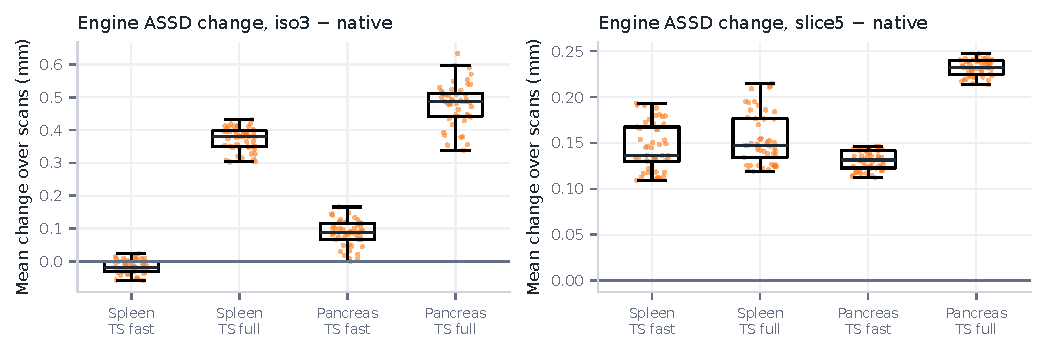
\includegraphics[width=0.85\textwidth]{configurations.pdf}
\caption{Mean change in engine ASSD from native to \lvl{iso3} (left) and \lvl{slice5} (right), one point per reconstruction configuration.}
\label{s:configs}
\end{figure*}

\begin{table*}[!t]
\caption{Engine conclusions across the 49 configurations: range of the mean ASSD change (mm), share of configurations with $|$change$|\leq0.05$\mm (\lvl{iso3}) or a positive change (\lvl{slice5}), and share where scans out-weigh resolution.}
\label{s:configtab}
\centering\footnotesize
\begin{tabular}{llrrrrrr}
\toprule
Organ & Engine & Configs & iso3 change range & $|$iso3$|\leq$0.05 & slice5 change range & slice5 $>$ 0 & Case $>$ resolution \\
\midrule
Spleen & TS fast & 49 & -0.059 to +0.025 & 90\% & +0.109 to +0.193 & 100\% & 100\% \\
 & TS full & 49 & +0.303 to +0.432 & 0\% & +0.119 to +0.215 & 100\% & 100\% \\
Pancreas & TS fast & 49 & +0.000 to +0.166 & 20\% & +0.112 to +0.146 & 100\% & 100\% \\
 & TS full & 49 & +0.338 to +0.633 & 0\% & +0.213 to +0.247 & 100\% & 100\% \\
\bottomrule
\end{tabular}

\end{table*}

\section{Engine repeatability}
\emph{Since the revision: does the same scan give the same mask?} Ten scans (five per organ, drawn with seed 2026) were segmented repeatedly in both modes: five times in one persistent GPU process, as the application runs the engine; three times in a new GPU process each, where nnU-Net's cuDNN autotuning may choose different kernels; and on the CPU, twice in fast mode and twice in full mode on one scan per organ. Each run is compared with the first run in the persistent process (Table~\ref{s:repeat}). The persistent process returned identical masks in every repeat. A new process or the CPU changed at most 96 organ voxels, which moved the mesh by at most 0.025\mm and its ASSD against the expert surface by at most 0.014\mm, an order of magnitude below the between-scan differences in the paper. Meshing the same mask twice gave identical meshes for all 590 meshes of S14.

\begin{table*}[!t]
\caption{Repeated segmentation against the first run in one persistent GPU process: runs, organ voxels changed and organ Dice (worst run), mesh shift (ASSD to the first run's mesh, max, mm), range of ASSD against the expert surface across repeats of one scan (max, mm), and median seconds per scan.}
\label{s:repeat}
\centering\footnotesize
\begin{tabular}{llrrrrrr}
\toprule
Mode & Path & Runs & Organ voxels & Dice & Mesh shift & ASSD range & Seconds \\
\midrule
fast & one persistent process & 40 & 0 & 1.0000 & 0.000 & 0.000 & 6 \\
 & new GPU process & 30 & 96 & 0.9993 & 0.017 & 0.014 & 30 \\
 & CPU & 20 & 96 & 0.9990 & 0.025 & 0.014 & 34 \\
full & one persistent process & 40 & 0 & 1.0000 & 0.000 & 0.000 & 18 \\
 & new GPU process & 30 & 16 & 0.9996 & 0.015 & 0.011 & 76 \\
 & CPU & 4 & 4 & 1.0000 & 0.002 & 0.006 & 175 \\
\bottomrule
\end{tabular}

\end{table*}

\section{An accuracy estimate per mesh}
\emph{Since the revision: can the results become an estimate shown with each mesh, and is it honest?} The application reports three figures with every mesh: the resolution limit, $0.177\,\Delta$ with $\Delta$ the RMS voxel spacing and a range of 0.13--0.21\,$\Delta$ from the Tier~1 floor; the shift its smoothing and decimation caused, measured against the mesh's own canonical surface; and, for the spleen and pancreas only, the engine's canonical ASSD from this study as a median, interquartile range (IQR) and 90\% range. Each was checked against the true error of the application's own meshes on all 82 scans, both modes and all four levels (590 meshes). On the held-out pancreas, 98\% of coarsened expert surfaces fell within $\pm0.111$\mm of $0.177\,\Delta$ (mean miss 0.029\mm); every delivered mesh was at least as far from the expert surface as its resolution limit; the measured smoothing shift matched the change it caused in signed distance within 0.022\mm (median); and the watertight flag agreed with VTK's edge classification for all 590 meshes.

The engine figure was checked leave one scan out (Table~\ref{s:card}, Fig.~\ref{s:cardfig}). Built from the native reference everywhere, with the paper's \lvl{slice5} change added on 5\mm grids (v1), its IQR held 46\% of delivered meshes overall but only 15\% of full-mode spleen meshes at \lvl{iso3}, where that mode degrades (S10). Taking the reference from the tested level closest to the scan's spacing (v2) brought this to 50\% overall and at least 44\% in every cell, with 86\% inside the 90\% range; empirical quartiles and 5--95\% ranges of 40 scans are expected to hold a new scan 48\% and 86\% of the time. The estimate is thus calibrated within each organ on the scans that define it; it does not transfer between organs (the spleen's 90\% range held 5\% of pancreas meshes), and other structures are reported as not validated.

\begin{table}[!t]
\caption{Share of delivered meshes (\%) whose ASSD against the expert surface fell inside the engine figure's IQR and 90\% range, leave one scan out. v1: native reference everywhere; v2: reference from the closest tested level.}
\label{s:card}
\centering\footnotesize
\setlength{\tabcolsep}{4pt}
\begin{tabular}{lllrrrr}
\toprule
Organ & Mode & Level & v1 IQR & v2 IQR & v1 90\% & v2 90\% \\
\midrule
spleen & fast & \texttt{native} & 49 & 56 & 90 & 90 \\
 &  & \texttt{iso1.5} & 44 & 44 & 78 & 78 \\
 &  & \texttt{iso3} & 37 & 46 & 71 & 76 \\
 &  & \texttt{slice5} & 43 & 50 & 57 & 86 \\
 & full & \texttt{native} & 61 & 63 & 93 & 93 \\
 &  & \texttt{iso1.5} & 54 & 54 & 93 & 93 \\
 &  & \texttt{iso3} & 15 & 46 & 56 & 90 \\
 &  & \texttt{slice5} & 36 & 50 & 79 & 93 \\
\midrule
pancreas & fast & \texttt{native} & 46 & 46 & 88 & 88 \\
 &  & \texttt{iso1.5} & 49 & 46 & 85 & 85 \\
 &  & \texttt{iso3} & 49 & 49 & 83 & 83 \\
 &  & \texttt{slice5} & 54 & 51 & 86 & 83 \\
 & full & \texttt{native} & 49 & 49 & 85 & 85 \\
 &  & \texttt{iso1.5} & 51 & 51 & 88 & 85 \\
 &  & \texttt{iso3} & 49 & 49 & 80 & 83 \\
 &  & \texttt{slice5} & 46 & 51 & 86 & 89 \\
\bottomrule
\end{tabular}

\end{table}

\begin{figure*}[!t]
\centering
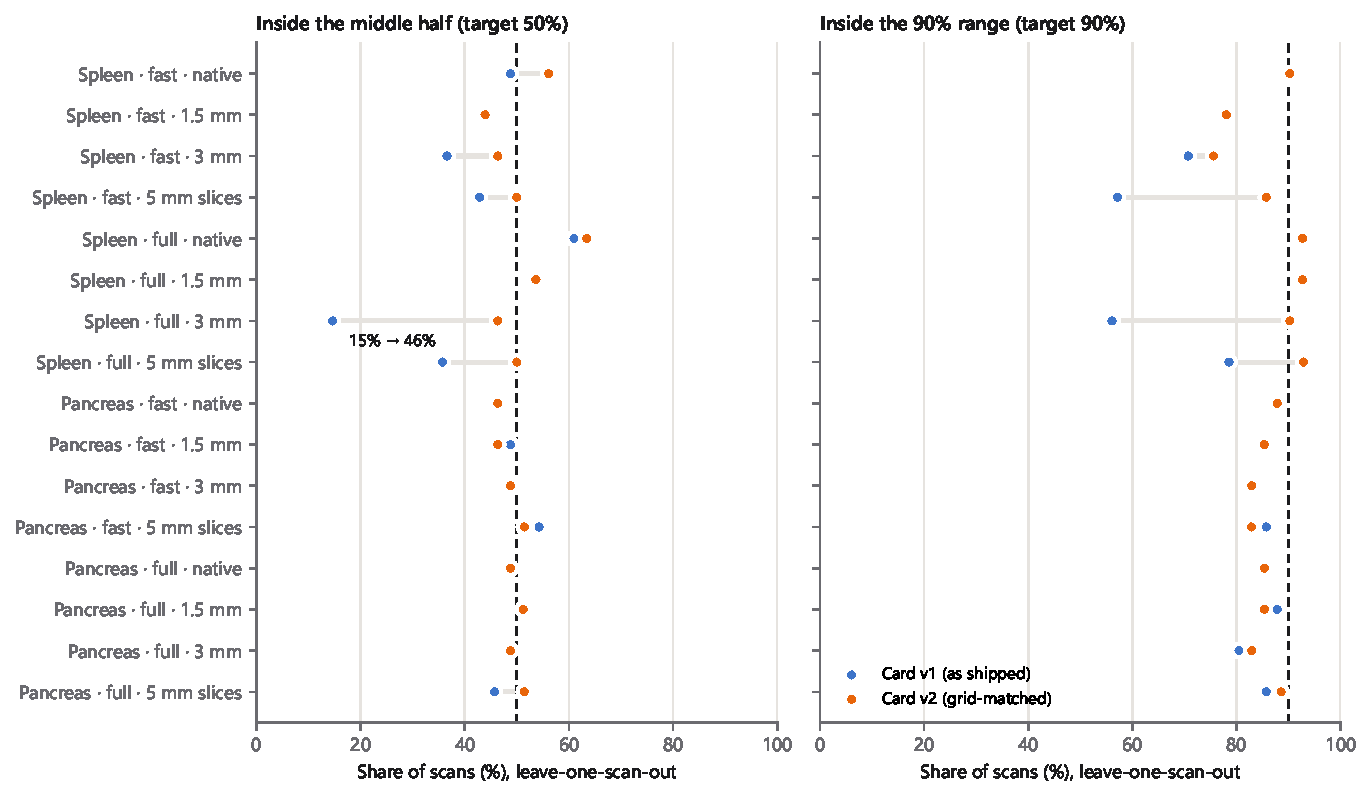
\includegraphics[width=0.85\textwidth]{card_coverage.pdf}
\caption{Coverage of the engine figure before (v1) and after (v2) matching it to the scan's grid, by organ, mode and level; dashed lines mark the targets.}
\label{s:cardfig}
\end{figure*}


\end{document}
